% ----------------------------------------------------------
\chapter{Introdução}\label{cap:introducao}
% ----------------------------------------------------------

Um objetivo comum no desenvolvimento de aeronaves é a redução do peso estrutural, pois influencia diretamente na carga paga útil carregada e, consequentemente, no desempenho de mercado do projeto. Por outro lado, tal redução pode estar associada com a redução da rigidez estrutural dos componentes do veículo. Como resultado, efeitos aeroelásticos afetam o comportamento dinâmico da aeronave e o desempenho em voo e, por isso, devem ser considerados no ciclo de projeto.

O estudo de aeroelasticidade, dividido nas subáreas de aeroelasticidade estática e dinâmica, auxilia na investigação da resposta da estrutura devido ao escoamento e na influência das deformações da estrutura nos carregamentos aerodinâmicos \cite{book:Wright-Cooper}. A subárea estática visa descrever as deformações estruturais resultantes de carregamentos aerodinâmicos em regime permanente e avalia fenômenos como a divergência e reversão de comando. Já a aeroelasticidade dinâmica investiga o movimento vibratório da estrutura na presença de variações temporais nas forças aerodinâmicas, tendo como objeto de estudo principal um fenômeno conhecido como \textit{flutter} \cite{art:Collar-1978, art:Garrick&Reed-1981}. O \textit{flutter} é caracterizado como uma instabilidade dinâmica da estrutura, cujo movimento apresenta auto-excitação, ocorrendo quando há o acoplamento dinâmico entre dois modos elásticos quaisquer do sistema \cite{book:Wright-Cooper, art:Sun-2014}. Movimentos oscilatórios da estrutura ocorrem para todas as velocidades de voo da aeronave. Contudo, a partir de uma determinada velocidade, esses movimentos aumentam de amplitude continuamente, caracterizando um movimento dinâmico instável. Tal velocidade é denominada velocidade de \textit{flutter} \cite{book:Wright-Cooper}.

Efeitos aeroelásticos afetam o desenvolvimento da aviação antes mesmo do primeiro voo de uma aeronave propelida acontecer. É discutido por \textcite{book:Bisplinghoff} que a causa atribuída à segunda falha do protótipo Aerodrome A, Figura \ref{fig:cap1:Aerodrom-Langley}, desenvolvido por Samuel Langley em 1903, ocorreu devido a problemas aeroelásticos, mais especificamente ao efeito de divergência. Problemas de divergência nas superfícies aerodinâmicas foram muito comuns durante os avanços da aviação durante a Primeira Guerra Mundial e, como abordado por \textcite{art:Collar-1978}, esses problemas eram solucionados simplesmente aumentando a rigidez estrutural.

\begin{figure}[ht]
    \centering
    \caption{Foto das tentativas de voo do protótipo Aerodrome A, no dia 07 de Outubro de 1903. Foram realizadas duas tentativas de voo, nas quais a aeronave foi catapultada de uma plataforma no rio Potomac, EUA. Em ambas tentativas o protótipo caiu no rio.}
    \noindent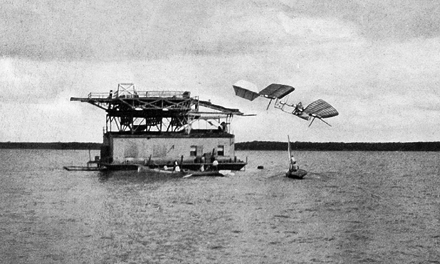
\includegraphics[width=\textwidth]{trabalho-graduacao/capitulos/figures/cap_1/Aerodrome-Langley.jpeg}
    \label{fig:cap1:Aerodrom-Langley}
\end{figure}

A primeira ocorrência documentada de \textit{flutter} afetando o voo de uma aeronave ocorreu em 1916 com o bombardeiro  Handley Page O/400 \cite{art:Le-2015}. Nesse caso, a aeronave apresentou oscilação extrema da empenagem, causando deformação da fuselagem e impactando a dinâmica do voo devido ao movimento dos profundores se tornarem assimétricos graças à deformação. Um exemplo de \textit{flutter} causando dano estrutural fora da aviação, é o colapso da ponte de Tacoma Narrows no dia 7 de Novembro de 1940 \cite{art:Billah-1990}. O fenômeno foi induzido por ventos de alta velocidade, chegando a aproximadamente $18,9$ m/s, o que levou a vibrações de extrema magnitude, como mostrado na Figura \ref{fig:cap1:Tacoma-Bridge}.

\begin{figure}[ht]
    \centering
    \caption{Fotos da ponte Tacoma Narrows, EUA colapsando em Novembro de 1940 devido ao \textit{flutter}; (\ref{fig:Tacoma-Oscilacao-01}) e (\ref{fig:Tacoma-Oscilacao-02}) mostram a amplitude das oscilações da seção central da ponte vista de cima, (\ref{fig:Tacoma-Oscilacao-03}) mostra a oscilação vista de fora da ponte, e (\ref{fig:Tacoma-Colapso}) apresenta uma foto após o colapso estrutural}
    \begin{subfigure}[t]{0.49\textwidth}
        \centering
        \caption{}
        \noindent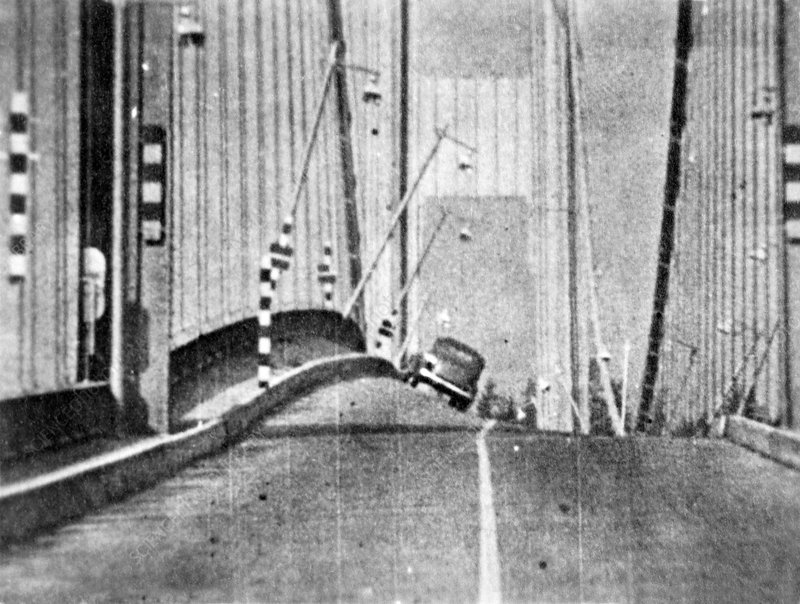
\includegraphics[width=\textwidth]{trabalho-graduacao/capitulos/figures/cap_1/Tacoma-Bridge-01.jpg}
        \label{fig:Tacoma-Oscilacao-01}
    \end{subfigure}
    \begin{subfigure}[t]{0.49\textwidth}
        \centering
        \caption{}
        \noindent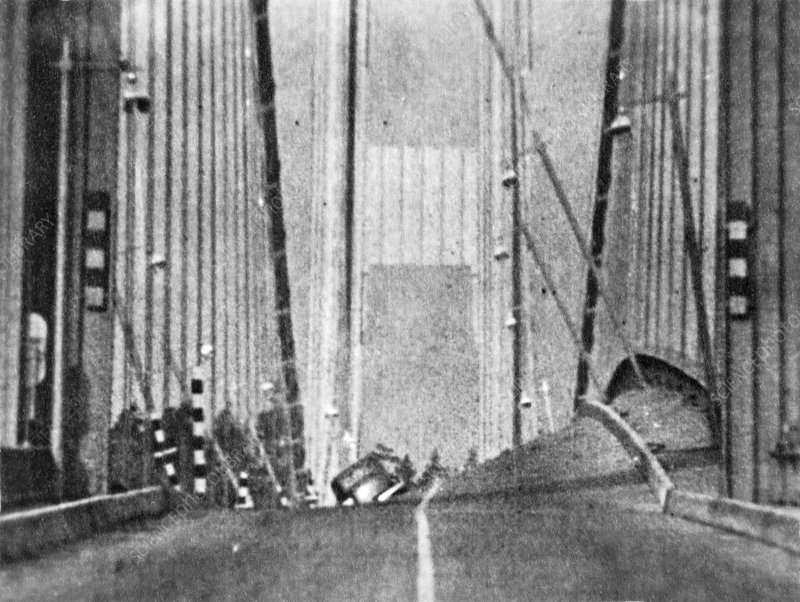
\includegraphics[width=\textwidth]{trabalho-graduacao/capitulos/figures/cap_1/Tacoma-Bridge-02.jpg}
        \label{fig:Tacoma-Oscilacao-02}
    \end{subfigure} \\
    \begin{subfigure}[t]{0.49\textwidth}
        \centering
        \noindent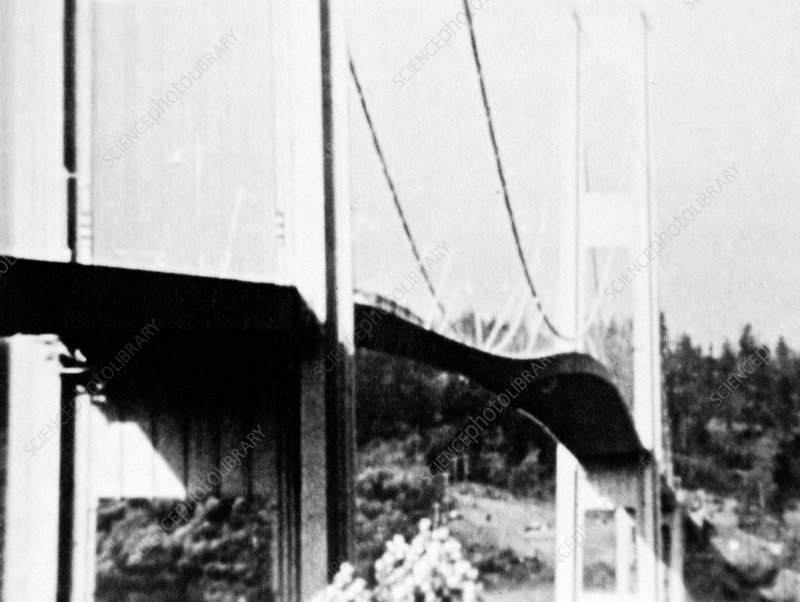
\includegraphics[width=\textwidth]{trabalho-graduacao/capitulos/figures/cap_1/Tacoma-Bridge-03.jpg}
        \caption{}
        \label{fig:Tacoma-Oscilacao-03}
    \end{subfigure}
    \begin{subfigure}[t]{0.49\textwidth}
        \centering
        \noindent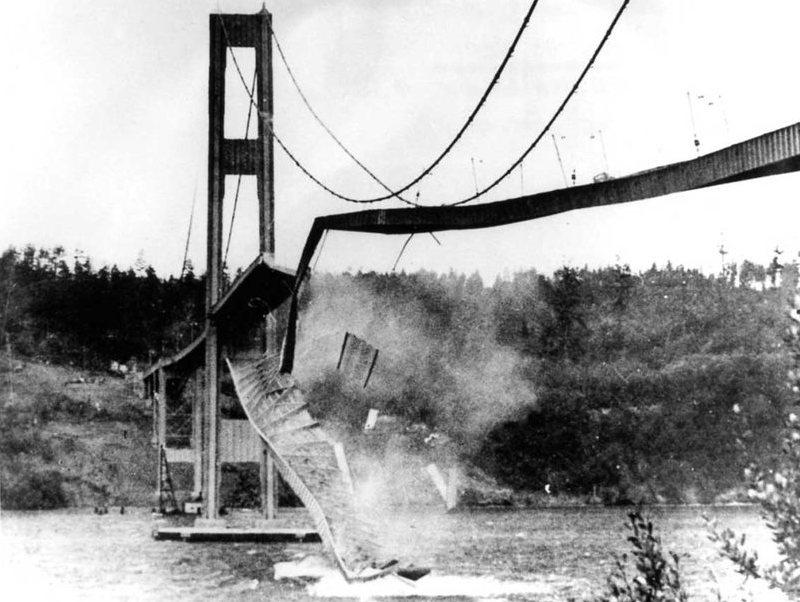
\includegraphics[width=\textwidth]{trabalho-graduacao/capitulos/figures/cap_1/Tacoma-Bridge-04.png}
        \caption{}
        \label{fig:Tacoma-Colapso}
    \end{subfigure}
        \label{fig:cap1:Tacoma-Bridge}
\end{figure}

Para evitar danos estruturais associados ao fenômeno do \textit{flutter}, restrições são consideradas no projeto aeronáutico visando impedir que a velocidade na qual essa instabilidade ocorre esteja dentro do envelope de operações, como, por exemplo, as restrições impostas pela \glsxtrfull{FAA} para projeto aeronáutico pelas normas 14 C.F.R § 23 e 25. Tais restrições se refletem no acréscimo de massa estrutural, afim de mitigar possíveis problemas encontrados no decorrer do desenvolvimento. Além disso, o envelope de voo é estritamente mantido para que a aeronave não se aproxime da velocidade de \textit{flutter} \cite{art:Sun-2014}. Com o objetivo de propor formas de mitigar os problemas decorrentes desse fenômeno, foram propostas na literatura técnicas de controle ativo para supressão de \textit{flutter}, \glsxtrfull{AFS}. O uso de \gls{AFS} em projetos aeronáuticos pode ser dado tanto no início do desenvolvimento, quanto em estágios mais avançados. Quando utilizado em etapas iniciais, essa técnica pode acarretar em redução do peso vazio projetado e melhoria no desempenho da aeronave \cite{art:Livne-1999}. Em projetos já em andamento, o \gls{AFS} pode ser utilizada visando evitar acréscimos de massa ou reprojeto estrutural e aerodinâmico, quando deparado com problemas aeroelásticos \cite{art:Livne-2018}.

O emprego de \gls{AFS} visa aumentar a velocidade na qual a instabilidade ocorre. Diversos trabalhos foram realizados visando investigar o desempenho de sistemas \gls{AFS} em melhorar a estabilidade do sistema. Em \textcite{art:Sun-2014}, um aumento de $30\%$ na velocidade de \textit{flutter} foi obtido em simulação, para um modelo aeroservoelástico (composição entre os modelos aeroelástico e do atuador) desenvolvido no domínio do tempo da asa de \textit{Goland}, conhecida na literatura. O sistema \gls{AFS} utilizado pelo autor é composto por uma superfície de controle alocada no bordo de fuga e foi projetado empregando o controle preditivo baseado em modelo. Investigações experimentais envolvendo o \textit{flutter}, utilizando ensaios em túnel de vento de uma asa, foram realizadas por \textcite{art:NASA1367}. Os resultados obtidos foram comparados com um modelo desenvolvido para a asa ensaiada no domínio do tempo empregando a técnica de \glsxtrfull{RFA} para inclusão dos termos aerodinâmicos. Foi observado pelo autor que a utilização da RFA possibilitou descrever adequadamente o comportamento dinâmico do sistema quando comparado com os resultados experimentais observados. Uma comparação entre resultados experimentais e de simulação também foi apresentada por \textcite{art:Huang-2015}, que obteve um aumento de $8\%$ na velocidade de \textit{flutter} para uma asa tridimensional com \gls{AFS}.

Nesse contexto, o presente trabalho envolve o desenvolvimento de um controlador para aumento da velocidade de \textit{flutter} de uma seção típica de aerofólio bidimensional. Com tal propósito, é realizado a modelagem matemática do sistema no domínio do tempo com uma representação no espaço de estados, sendo os esforços aerodinâmicos incluídos no modelo a partir da técnica \gls{RFA} \cite{book:Wright-Cooper, art:NASA1367, art:NASA2776, art:RogerRFA1977}. A lei de controle para supressão de \textit{flutter} foi do tipo realimentação de estados, sendo o vetor de realimentação projetado utilizando o conhecido regulador linear quadrático, \glsxtrfull{LQR}. Nesta estratégia, o controlador é projetado de modo a minimizar uma função de custo quadrática composta pelo desvio dos estados da sua posição regulada e da maginute da ação de controle, considerando um modelo linear do sistema. Para o caso particular de tempo final infinito, a solução do problema do \gls{LQR} é um vetor de realimentação de estados, que é calculado a partir da equação de Riccati, e depende de matrizes de ajuste que ponderam entre a velocidade de resposta e o esforço de controle \cite{book:Franklin}. É possível demonstrar que tal técnica de projeto resulta em margens de estabilidade interessantes. Mais precisamente, o \gls{LQR} resulta em uma margem de ganho acima de 6 dB e de fase de $60^{\circ}$ \cite{art:Anderson-1966, book:Anderson-1971}, justificando o emprego dessa abordagem.

Diante do exposto, o restante do trabalho foi dividido e será apresentado no decorrer do presente relatório seguindo a divisão em quatro partes, sendo:

\begin{itemize}
    \item O Capítulo 2 abordará a descrição do sistema aeroservoelástico e o desenvolvimento matemático do modelo. Incluir-se-ão os modos aeroelásticos associados aos \glsxtrfull{GDLs} para avaliar as margens de estabilidade do sistema;
    \item Em seguida, no Capítulo 3, o desenvolvimento da lei de controle por realimentação de estado será apresentado;
    \item No Capítulo 4 serão apresentados os resultados de simulação, discutindo-se a eficácia da abordagem da lei de controle na supressão de \textit{flutter};
    \item Por fim, no Capítulo 5 são listadas as conclusões das investigações numéricas e elencadas propostas de trabalhos futuros para continuidade do desenvolvimento.
\end{itemize}

% ----------------------------------------------------------
